% Koma-Script class has better defaults for us, let's use it!
% https://mirrors.nic.cz/tex-archive/macros/latex/contrib/koma-script/doc/scrguien.pdf
% https://tex.stackexchange.com/questions/73248/what-packages-are-incompatible-with-koma-script

% Two sided book, chapter can begin on both left and right page
\documentclass[paper=b5,parskip=half,open=any,headsepline=true,11pt]{scrbook}

% Number pages to header
% https://tex.stackexchange.com/a/278627/220596
\usepackage[automark]{scrlayer-scrpage}
\clearpairofpagestyles
\ohead{\headmark}
\ihead*{\pagemark}

% The toolbox package allows us to use conditional compilation, so we can get colored and black-and-white versions from the same source
\usepackage{etoolbox}

% all includes and settings are in a separate file
% This document needs to be compiled by XeLaTeX
% https://www.overleaf.com/learn/latex/XeLaTeX

% XeTeX options inspired by: https://www.fi.muni.cz/lemma/PB029/practices/ceska-sazba-texem/files/xelatex.tex
\usepackage{polyglossia}
\setdefaultlanguage{english}
% \def\uv#1{„#1“}

% TODO: Figure out why -- is not turned to ndash :-(
\usepackage{fontspec}
\defaultfontfeatures{Scale=MatchLowercase,Mapping=tex-text}

\usepackage{amsmath}
\usepackage{mathtools}  % Needed for rightcentered pmatrix* in symetrie.tex
% Math-style ISO turns capital greek letters italic
% \usepackage[math-style=ISO,warnings-off={mathtools-colon,mathtools-overbracket}]{unicode-math}
\usepackage{realscripts}
\usepackage{graphicx}
\usepackage{csquotes}
\usepackage{lscape}     % Landscape orientace pro velké tabulky
\usepackage{braket}
\usepackage{xcolor}
\usepackage{bm} % bold greek letters
\usepackage{mathrsfs}

% library
\usepackage[style=chem-acs]{biblatex} % bibliography
\addbibresource{library.bib}

% https://www.overleaf.com/learn/latex/Questions/Which%20OTF%20or%20TTF%20fonts%20are%20supported%20via%20fontspec%3F#Latin-script_Fonts
% Font sampler: https://www.overleaf.com/articles/fontspec-all-the-fonts/hjrpnxhrrtxc
% font recommendations https://practicaltypography.com/free-fonts.html
\usepackage{lmodern} % this is loaded by default in unicode-math
\setmainfont{IBM Plex Serif}
\setsansfont{IBM Plex Sans}
\setmonofont{IBM Plex Mono}
\setmonofont{Source Code Pro}
% Needs unicode-math
% \setmathfont{Asana Math}


% http://latexcolor.com/
\usepackage{xcolor}
\colorlet{ourcyan}{cyan!10}
\colorlet{darkercyan}{cyan!70}
\definecolor{wine}{HTML}{722f37}
\definecolor{persianplum}{HTML}{701c1c}
% Barevné nadpisy
\setkomafont{disposition}{\color{persianplum}\bfseries}

% packages and setting for code formating
\usepackage{listings} % https://www.overleaf.com/learn/latex/Code_listing
\definecolor{codegreen}{rgb}{0,0.6,0}
\definecolor{codegray}{rgb}{0.5,0.5,0.5}
\definecolor{codepurple}{rgb}{0.58,0,0.82}
\definecolor{codeblue}{rgb}{0,0.5,1}
\definecolor{codeorange}{rgb}{1,0.5,0}
\definecolor{backcolour}{rgb}{0.95,0.95,0.92}

%\lstset{
%  basicstyle=\ttfamily,
%  backgroundcolor=\color{backcolour},   
%}

\lstdefinestyle{mystyle}{
    backgroundcolor=\color{backcolour},   
    commentstyle=\color{codegreen},
    keywordstyle=\color{codeorange},
    numberstyle=\tiny\color{codegray},
    stringstyle=\color{codeblue},
    basicstyle=\ttfamily\footnotesize,
    breakatwhitespace=false,         
    breaklines=true,                 
    captionpos=b,                    
    keepspaces=true,                 
    numbers=left,                    
    numbersep=5pt, 
    frame=single,  % remove this keyword to remove frame
    showspaces=false,                
    showstringspaces=false,
    showtabs=false,                  
    tabsize=2
}
\lstset{style=mystyle}

\lstdefinestyle{mystyle2}{
    backgroundcolor=\color{backcolour},   
    commentstyle=\color{codegreen},
    keywordstyle=\color{codeorange},
    %numberstyle=\tiny\color{codegray},
    stringstyle=\color{codeblue},
    basicstyle=\ttfamily\normalsize,
    breakatwhitespace=false,         
    breaklines=true,                 
    captionpos=b,                    
    keepspaces=true,                 
    numbers=none,                    
    numbersep=5pt,       
    frame=single, % remove this keyword to remove frame
    showspaces=false,                
    showstringspaces=false,
    showtabs=false,                  
    tabsize=2
}

\lstdefinestyle{bash}{
    backgroundcolor=\color{backcolour},   
    commentstyle=\color{codegreen},
    keywordstyle=\color{codeblack},
    %numberstyle=\tiny\color{codegray},
    stringstyle=\color{codeblue},
    % basicstyle=\sffamily\normalsize,
    breakatwhitespace=false,         
    breaklines=true,                 
    captionpos=b,                    
    keepspaces=true,                 
    % numbers=false,                    
    numbersep=5pt,                  
    showspaces=false,                
    showstringspaces=false,
    showtabs=false,                  
    tabsize=2,
    prebreak=\raisebox{-1ex}[0ex][0ex]{\color{codeorange}\ensuremath{\hookleftarrow}}
}
\newcommand\bash[1]{\colorbox{backcolour}{\lstinline[language=bash,style=bash]{#1}}} 
\newcommand\python[1]{\colorbox{backcolour}{\lstinline[language=bash,style=mystyle2]{#1}}} 


% Better footnote positioning
% https://mirrors.nic.cz/tex-archive/macros/latex/contrib/footmisc/footmisc.pdf
% Odsazeni footnote od horizontální čáry
\addtolength{\footnotesep}{2pt}
% Větší odsazení footnote od hlavního textu
% https://tex.stackexchange.com/questions/371138/change-space-between-footnote-line-and-main-text
\addtolength{\skip\footins}{8pt plus 4pt}
\usepackage[hang]{footmisc}
\setlength{\footnotemargin}{2mm}

% Inline fractions
\newcommand{\nicefrac}[2]{#1/#2}
% TODO: get rid of nicefrac in favour of inline frac
\newcommand{\inlinefrac}[2]{#1/#2}

% sazeni jednotek
\usepackage{siunitx}
\sisetup{
exponent-product = \cdot,
inter-unit-product = \, ,
%inter-unit-product = \ensuremath{{}\cdot{}},
output-decimal-marker = {,},
group-separator = \,,
group-minimum-digits = 4
}
\DeclareSIUnit{\kcal}{kcal}
\DeclareSIUnit{\ev}{eV}
\DeclareSIUnit{\eV}{eV}
\DeclareSIUnit{\angstrom}{Å}

% Vylepseni tabulek
\usepackage{multicol} % slouceni sloupcu v tabulce
\usepackage{multirow} % slouceni radku v tabulce
\usepackage{rotating} % rotace tabulky
\usepackage{booktabs} % lepsi vzhled tabulek

\usepackage[version=4]{mhchem} % sázení chemických vzorců
% Maybe we could use this for MO diagrams!
% https://www.overleaf.com/learn/latex/Molecular_orbital_diagrams
% \usepackage{MODiagram}

% puntik radikalu 
\usepackage{chemformula}


% here is a nice documentation for tcolorbox
% https://www.overleaf.com/latex/examples/drawing-coloured-boxes-using-colorbox/pvknncpjyfbp#.VmjpHx8SprQ1
\usepackage{tcolorbox}
\tcbuselibrary{breakable,skins} %boxes over more pages

%%%%%%% DEFINICE BOXIKU %%%%%%
\newenvironment{ourbox}[1]
{
\medskip
\begin{tcolorbox}[breakable,width=\textwidth,title={\sffamily \large \textbf{#1}},colback=cyan!5!white,colframe=cyan!80!black, coltitle=white,boxrule=0.25mm,toptitle=1mm,bottomtitle=1mm]
}
{
\end{tcolorbox}
}

\newenvironment{ourbox-BW}[1]
{
\medskip
\begin{tcolorbox}[breakable,width=\textwidth,title={\sffamily \large \textbf{#1}},colback=gray!20!white,colframe=black, coltitle=white,boxrule=0.25mm,toptitle=1mm,bottomtitle=1mm]
}
{
\end{tcolorbox}
}

%%%%%%%%%%%%%%%%%%%%%%%%%%%%%%

% https://www.overleaf.com/learn/latex/page_size_and_margins
% http://mirrors.ibiblio.org/CTAN/macros/latex/contrib/geometry/geometry.pdf
% \usepackage[ paperheight = 240mm, paperwidth = 170mm,  % or: "paper=a4paper"
\usepackage[ paperheight = 297mm, paperwidth = 210mm,  % or: "paper=a4paper"
             % layoutheight = 200mm, layoutwidth = 138mm,
             % layoutvoffset = 12mm, layouthoffset = 16mm,
             % margin=0pt,
             left = 20mm,
             right = 20mm,
             top = 25mm,
             bottom = 25mm,
             footskip = 24pt,
             marginparwidth=0pt,
             marginparsep=0pt,
             headheight=8mm,
             headsep=7pt,
             showframe = false, showcrop = false]{geometry}


% Popisky obrazku a tabulek
% http://ftp.cvut.cz/tex-archive/macros/latex/contrib/caption/caption-eng.pdf
\usepackage{caption}   
\captionsetup{labelfont=bf}         % tucne "Obr." a "Tab.'
\captionsetup{format=plain}         % normal par justification
\captionsetup{width=0.9\textwidth}  % úprava šířky popisků
\captionsetup{font=small}           % mensi font u popisku
\captionsetup[figure]{name=Obr.}

% Vektory tucne a ne italikou
% definice fungujici i pro recke symboly, viz
% https://tex.stackexchange.com/questions/3535/bold-math-automatic-choice-between-mathbf-and-boldsymbol-for-latin-and-greek
%\renewcommand{\vec}[1]{\boldsymbol{\mathbf{#1}}}

% Vektory Bold, sans-serif, italic (jako v Atkinsovi)
% Unicode math redefines\vec at beginning of document! Hence this, per:
% https://tex.stackexchange.com/a/457845
% symbssfit per unicode-math documentation

% Vektory tucnou kurzivou!!!
% \AtBeginDocument{\renewcommand{\vec}[1]{\symbfsfit{#1}}}
% \renewcommand{\boldsymbol}[1]{\symbf{#1}}

% prikaz na vykresleni diferencialu
% from http://tex.stackexchange.com/questions/60545/should-i-mathrm-the-d-in-my-integrals
\newcommand\dd{\mathop{}\!\mathrm{d}} 

% zkrácený výraz pro parciální derivaci
\newcommand{\pd}{\partial}

\usepackage{svg}
\usepackage{capt-of}

\newcommand{\dv}[2]{\frac{\dd #1}{\dd #2}}
\newcommand{\ddv}[2]{\frac{\dd^2 #1}{\dd #2^2}}


% zkraceny vyraz pro hmotnost elektronu
\newcommand{\me}{m_{\mathrm{e}}}

% magnetické spinové číslo elektronu
\newcommand{\ms}{m_{\mathrm{s}}}
\newcommand{\msi}[1]{m_{\mathrm{s}#1}}

% zkraceny vyraz pro exponencialu
\newcommand{\ee}{\mathrm{e}}

% Stojate pi
% https://tex.stackexchange.com/questions/219975/how-to-get-non-italic-greek-symbols-with-ams-packages
% Somehow this does not seem to work, probably because of unicode-math
% \renewcommand{\pi}{\uppi}

% Kdyz takto mame exponencialu, tak stejne by mela byt imaginarni jednotka
% https://tex.stackexchange.com/questions/86128/how-should-imaginary-numbers-be-typeset
%\newcommand{\ii}{i}
\newcommand{\ii}{\mathrm{i}}
\newcommand{\e}{\mathrm{e}}


%Kolafova zavorka pres 3 radky
\newcommand*\twobrace{$\displaystyle\left.\rule{0pt}{3.1ex}\right\}$}
\newcommand*\threebrace{$\displaystyle\left.\rule{0pt}{5ex}\right\}$}


% procedura definujici nove prostredi "priklad"
%%%%%%%%%%%%%%%%%%%%%%%%%%%%%%%%%%%
% Autor: Vit Svoboda, Praha 2014
%%%%%%%%%%%%%%%%%%%%%%%%%%%%%%%%%%%
\newcounter{poradi} % novy citac pro cislo prikladu
\newcounter{CP} % novy citac pro cislo v labelu
\newcommand{\novepocitadlo}{\stepcounter{poradi}\theporadi} % realizace pocitadla pro cislo prikladu 
\newcommand{\prikladlabel}[1]{\refstepcounter{CP}\label{#1}} % novy prikaz pro label, ktery resi spravny odkaz \ref

%prikaz, který vypise "Priklad xy"
\definecolor{bleudefrance}{rgb}{0.19, 0.55, 0.91}
\newcommand{\novynadpis}{
{
  \color{bleudefrance}
  \normalsize \sffamily {Exercise \novepocitadlo}
} 
  \vspace{0.1cm} \prikladlabel{\theporadi}
} 

\newenvironment{priklad}
{
\vspace{4pt plus 2pt}
\begin{tcolorbox}[
empty,
breakable,
%colback=white,
%colbacktitle=white,
%colframe=gray,
%boxrule=0pt,
borderline west={1.5pt}{0pt}{gray}
]
\novynadpis\\ \noindent
}
{
\end{tcolorbox}
\vspace{4pt plus 2pt}
}
%%%%%%%%%%%%%%%%%%%%%%%%%%%%%%%%%%%%

% cislovani rovnic, obrazku a prikladu v kazde sekci zvlast
\numberwithin{equation}{chapter} 
\numberwithin{figure}{chapter}
\numberwithin{poradi}{chapter}
\numberwithin{CP}{chapter}
\graphicspath{{obrazky/}{../obrazky/}} % adresar pro obrazky

% kontrola vdov a sirotku
% defaultlines=2 is latex default
\usepackage[defaultlines=2,all]{nowidow}

%lepsi pozicovani
\usepackage{float}

\usepackage{url}   %pro snadnou tvorbu URL adres

\usepackage[shortcuts]{extdash}

\usepackage[
unicode,
xetex,
pdfa=true,
pdfencoding=unicode,
unicode=true,
pdftitle={Quantum Mechanics: Hands On},
pdfauthor={Jiří Janoš, Tomáš Jíra},
colorlinks=true,
bookmarks=true,
breaklinks=true,
urlcolor=blue,
citecolor=blue,
linkcolor=blue,
unicode=true,
pdfstartview=FitV]{hyperref}


%/nastaveni VZHLEDU PROGRAMOVACÍCH JAZYKŮ
% See https://cs.overleaf.com/learn/latex/Code_listing
% nasledujici styl nema keywords ani jinou syntax,
% vlastně je to jen verbatim prostředí s šedým pozadím
% TODO: asi by se dalo udělat jednodušeji bez lstlistings
\usepackage{listings}
\lstdefinestyle{bezsyntaxe}{
    basicstyle=\ttfamily,
    backgroundcolor=\color{gray!15},
    frameround=fttt,
    breaklines=true,
    tabsize=5,
    frame=tb, % lines above and below 
    framexleftmargin=3pt,
    framextopmargin=4pt,
    framexbottommargin=4pt, 
    framerule=1pt,
    rulecolor=\color{gray!15}, % colored in a slightly darker gray
    breakatwhitespace=true,
    numbers=none,
    sensitive=false,
    showstringspaces=false,
  %  comment=[l]{\#},
}

% Not sure if we want this. No margin for lists
% https://tex.stackexchange.com/questions/295153/vertical-spacing-in-koma-script
\usepackage{enumitem}
\setlist{leftmargin=*}
% This is to get rid of the warning
% https://tex.stackexchange.com/a/514194
\setlist{labelwidth=*}

\usepackage{attachfile} % embedding files in PDF



% https://www.overleaf.com/learn/latex/Glossaries#Acronyms
% just \printglossary as described broke so I used fix introduced herehttps://stackoverflow.com/questions/66924808/unable-to-show-the-glossary-with-printglossary-in-latex
\usepackage[acronym]{glossaries}
% \makeglossaries
\makenoidxglossaries

% https://www.overleaf.com/learn/latex/Glossaries#Acronyms
\usepackage[acronym]{glossaries}
\makeglossaries
\newacronym{cc}{CC}{Coupled Cluster}
\newacronym{ci}{CI}{Configuration Interaction}
\newacronym{mp}{MP}{Møller--Plesset}
\newacronym{hf}{HF}{Hartree--Fock}
\newacronym{tdse}{TDSE}{time-dependent Schrödinger equation}
\newacronym{ft}{FT}{Fourier transform}
\newacronym{ift}{IFT}{inverse Fourier transform}

% https://www.overleaf.com/learn/latex/Indices
\usepackage{imakeidx}
\makeindex

% custom hyphenation of words
\hyphenation{Har-tree-ho}
\hyphenation{Har-tree}
\hyphenation{Fock-ových}
\hyphenation{Kohn-ových}
\hyphenation{Fock-ovy}
% Not sure here, but we're overflowing to margin in historie.tex
\hyphenation{Fra-nck}
\hyphenation{Oppen-heimer-ova}
\hyphenation{Oppen-heimer}
\hyphenation{Born-ova}
\hyphenation{Uvaž-me}
\hyphenation{dis-perz-ní}
\hyphenation{disp-erze}
\hyphenation{kva-dru-pól}
\hyphenation{di-pól}
\hyphenation{di-pól}
\hyphenation{kvan-to-vě}
\hyphenation{mole-ku-lár-ně}
\hyphenation{ne-glect}
\hyphenation{or-to-go-nál-ní}
\hyphenation{Max-well-ových}

\usepackage{subcaption}

\title{Quantum Mechanics: Hands on}
\author{Jiří Janoš, Tomáš Jíra}

%%%%%%%%%%%%%%%%%%
% BEGIN DOCUMENT %
%%%%%%%%%%%%%%%%%%
\begin{document}
\frontmatter
\pagestyle{scrheadings}

% TITULNI STRANA
\begin{titlepage}
\begin{center}
\vspace*{2cm}
{\Huge \textbf{Quantum Mechanics in Chemistry:\\Hands on}}

\bigskip

\begin{figure} [H]
\centering
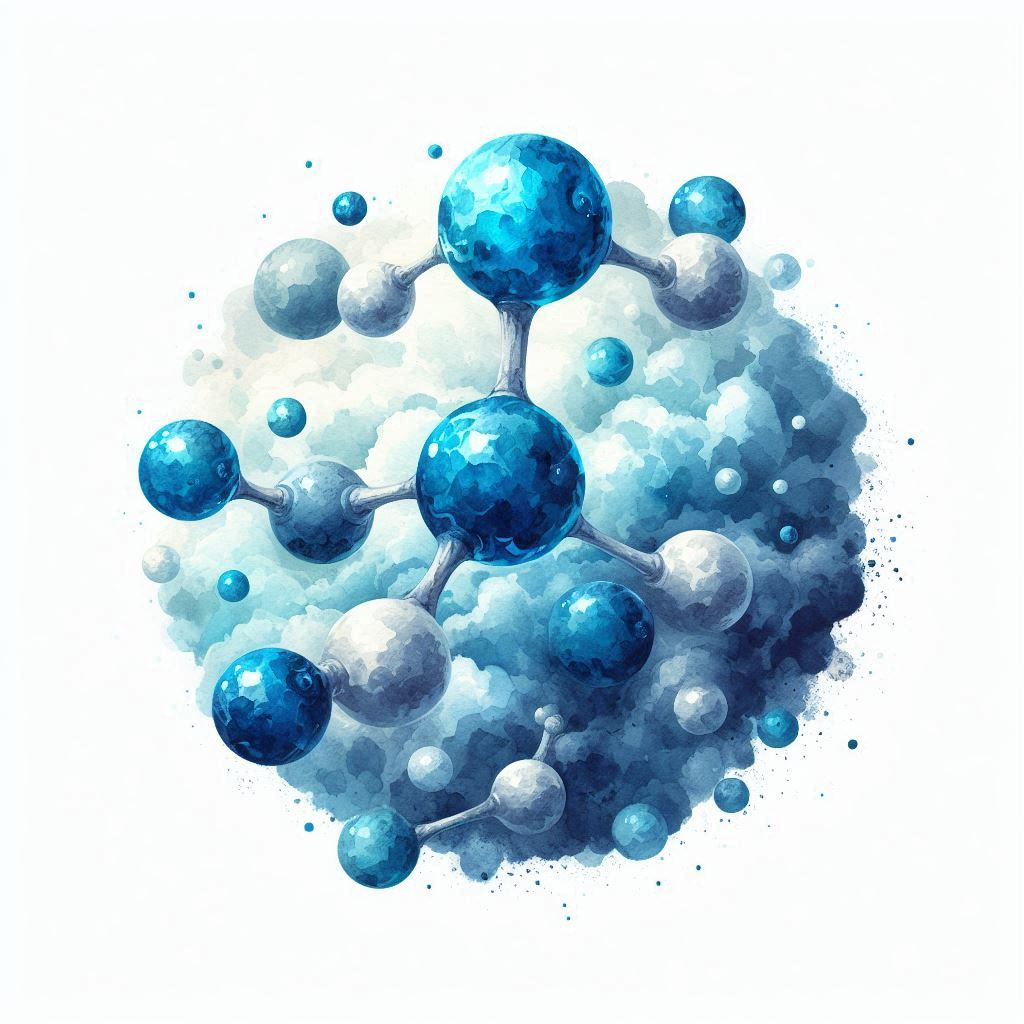
\includegraphics[width=0.7\textwidth]{cover2.jpg}
\end{figure}
\rule{0.8\textwidth}{0.02cm}\\

Jiří Janoš, Tomáš Jíra\\

\end{center}
\vfill
\begin{flushright}
\rule{3cm}{0.01cm} \\
Created in \LaTeX \\
\copyright \hspace{0.1cm} Prague 2024 \\
Version from \today
%\vspace{2cm}
\end{flushright}
\end{titlepage}
% Nasledující v tuto chvíli není potřeba, je uděláno automaticky pomocí \frontmatter
%\pagestyle{plain}
%\pagenumbering{roman}
%\setcounter{page}{3}

% OBSAH
\tableofcontents

\chapter{Introduction}
\label{kap:uvod}
Lets code everything!

\section{Brief introduction to Python}
\subsection{Importing packages}
\begin{lstlisting}[language=Python, style=mystyle2]
import numpy as np
\end{lstlisting}

\mainmatter

\chapter{Hartree--Fock method}
\label{kap:hf}
\acrfull{hf} method 

\chapter{Quantum dynamics}
\label{kap:qd}
Up to this point, we have taken the time-independent perspective on quantum mechanics, focusing on methods for calculating stationary states of electrons in molecules. In this chapter, we shift to time-dependent quantum mechanics and look at the time evolution of quantum systems. We will focus on simple low-dimensional models and introduce a simple numerical scheme suitable for wave function propagation. The power of simple low-dimensional models resides in the conceptual understanding of time evolution in quantum mechanics: they allow us to examine dynamics such as interference of two wave packets, tunnelling through energy barriers, or reflection of the wave packet on boundaries.

\section{Theoretical background}
\label{sec:qdtheoback}

The time evolution in quantum mechanics is governed by the \acrfull{tdse},
\begin{equation}
    i\hbar\frac{\dd\psi(x,t)}{\dd t} = \hat{H}(x)\psi(x,t) \, ,
    \label{eq:tdse}
\end{equation}
where $i$ is the imaginary unit, $\hbar$ is the reduced Planck constant, $\psi$ is the wave function, $\hat{H}$ is the Hamiltonian, $t$ is time and $x$ represents the position of a quantum particle, such as an electron, proton, or any other particle. The solution of the \acrshort{tdse} can be in general written as
\begin{equation}
    \psi(x,t) = \hat{U}(t)\psi(x,0) \, .
    \label{eq:U}
\end{equation}
The operator $\hat{U}$ is called a \textit{propagator} or \textit{time evolution operator}. Application of the propagator to a wave function is equivalent to evolving the wave function from time 0 to time t. The knowledge of the evolution operator is, therefore, elementary for a description of dynamics in quantum systems.

The propagator is easy to find if the Hamiltonian $\hat{H}$ does not depend on time. Then, we can formally write a solution of equation~\eqref{eq:tdse} in the following form:
\begin{equation}
    \psi(x,t) = \e^{-\frac{i}{\hbar}\hat{H}(x)t} \psi(x,0)\, .
    \label{eq:tdse2}
\end{equation}
Notice that the result resembles the separation of variables for differential equations, only for a equation with operators. Considering the Hamiltonian to be time-independent restricts the validity of equation~\eqref{eq:tdse2} only for systems without any time-dependent interaction such as oscillating electromagnetic field (radiation), collisions between particles, etc. The solution for time-dependent Hamiltonian is somewhat more complicated and will be omitted here.

Comparing equations~\eqref{eq:tdse2} and \eqref{eq:U}, we see that the evolution operator has a simple form of an exponential of the Hamiltonian,
\begin{equation}
    \hat{U}(t) = \e^{-\frac{i}{\hbar}\hat{H}(x)t} \, .
    \label{eq:U1}
\end{equation}
Formally, we now have a propagator containing all information about the time evolution of the system and we can propagate the wave function to an arbitrary time $t$. While this works well on paper, analytical evaluation of the propagator is in practice not a straightforward task for most Hamiltonians. The hindrance lies in the evaluation of the exponential in equation~\eqref{eq:U1}.

Let us briefly discuss why analytic evaluation of the exponential of Hamiltonian is a cumbersome task. The exponential of an operator is defined through its Taylor series as
\begin{equation}
    \e^{\hat{A}} = \sum_{l=0}^\infty \frac{\hat{A}^l}{l!} \, ,
\end{equation}
where $\hat{A}$ is and arbitrary operator. In our case, $\hat{A} = -\frac{i}{\hbar}\hat{H}(x)t$ which leads to the following relation:
\begin{equation}
    \hat{U}(t) = \sum_{l=0}^\infty \frac{\hat{H}^l}{l!} \left( -\frac{i}{\hbar} t\right)^l \, .
    \label{eq:U2}
\end{equation}
Considering the Hamiltonian in the standard form,
\begin{equation}
    \hat{H}(x) = \hat{T} + \hat{V}(x) = -\frac{\hbar^2}{2m}\frac{\dd^2}{\dd x^2} + V(x)\, ,
    \label{eq:Ham1}
\end{equation}
where $\hat{T}$ represents the kinetic energy operator, $\hat{V}$ stands for the potential energy operator and $m$ is the particle mass, the propagator becomes:
\begin{equation}
    \hat{U}(t) = \sum_{l=0}^\infty \frac{(\hat{T}+\hat{V})^l}{l!} \left( -\frac{i}{\hbar} t\right)^l \, .
    \label{eq:U3}
\end{equation}
Calculating this propagator requires computing an infinite series of powers of the Hamiltonian, further complicated by the fact that $\hat{T}$ and $\hat{V}$ do not commute and the exponential cannot be factorized. This makes direct evaluation infeasible for most of the potential.

Thus, analytical solutions of the \acrshort{tdse} are used only in model systems, usually when the complete basis of the respective Hilbert space is known. Instead, most time-dependent problems are solved numerically where arbitrary Hamiltonians are possible. 

\section{Numerical solution}

Systems of chemical interest span, in general, an infinite Hilbert space. In other words, an infinite number of orthogonal basis functions are required to fully represent the wave function of such a system. However, any computer can only handle a finite basis set, since computer memory is finite, and often even quite limited. Thus, in any numerical implementation of quantum mechanics, we work in a truncated basis set. This basis truncation is the first and fundamental source of error for any computer simulation. There are other sources of error due to the numeric schemes employed, e.g. trapezoid rule for integration, or due to a finite time step in our propagation. While these sources of error can be eliminated by improving our numeric schemes or the time step, the truncation error will be always present and dependent on how much we truncated our basis.
% consider reformulating the fundamental error and other errors

In this text, we will represent the system on a grid of discrete points, a natural representation for a computer. These grid points (we can think of them as a set of Dirac $\delta$-distributions) form our truncated basis set commonly referred to as a \textit{pseudospectral} basis. 
In the following, we will explain how to work with such a representation, including how to evaluate the action of an operator and calculate the expectation value. In the end, the flow of the text will lead us to the evolution operator $\hat{U}(t)$ and techniques for efficient propagation of the wave function.

\subsection{Representing wave function on a grid: the \textit{pseudospectral} basis}

As stated above we will work in a truncated \textit{pseudospectral} basis and represent the system with a set of $N$ discrete points. Since we work as usual in chemistry in the position representation, we start with discretizing the position coordinate $x$ and replacing it by a set of points:
\begin{align}
    x &\rightarrow \{x_0, x_1, x_2, \dots, x_N\} \, .
\end{align}
It is convenient for numerical applications to make the grid equidistant, meaning that the distance between any two neighbouring grid points, $\Delta x = x_i - x_{i-1}$, remains constant. 

Next, we express the wave function $\psi$ on this grid by evaluating it at each grid point $x_i$, giving:
\begin{align}
    \psi(x,t) &\rightarrow \{\psi(x_0,t), \psi(x_1,t), \psi(x_2,t), \dots, \psi(x_N,t)\} =  \{\psi_{0,t}, \psi_{1,t}, \psi_{2,t}, \dots, \psi_{N,t}\} \, .
\end{align}
We have now two indexes of $\psi$: the grid point index $i$ and time index $t$. Further in the text, we will drop the index $t$ to simplify the notation unless $\psi$ in two different times will appear in the equation.

Having the wave function defined on a grid, the next step is to compute its norm. In the position representation, the norm is an integral of $\psi^*\psi$ over the position $x$, which can be numerically realized for example by the trapezoidal rule:
\begin{equation}
    \langle \psi(x,t) | \psi(x,t) \rangle = \int_{-\infty}^\infty \psi^*(x,t)\psi(x,t) \dd x = \sum_{j=1}^N \frac{\psi^*_{j-1}\psi_{j-1} + \psi^*_{j}\psi_{j}}{2} \Delta x \, .
\end{equation}
While the trapezoidal rule is a simple and commonly used method, more accurate numerical integration schemes can be employed to reduce integration errors, though these may come at the cost of increased computational effort.

With the wave function defined, our attention now turns to operators: how to represent them and how to apply them. We will start with operators dependent only on the position $x$ since they are simple to represent on the grid. Take the potential energy operator $V(x)$ which can be represented on the grid similarly to the wave function as
\begin{align}
    V(x) &\rightarrow \{V(x_0), V(x_1), V(x_2), \dots, V(x_N)\} = \{V_0, V_1, V_2, \dots, V_N\} \, .
\end{align}
Now, applying the potential energy operator to the wave function reduces to a simple multiplication of the discretized operator and wave function as 
\begin{align}
    \hat{V}\psi &\rightarrow \{V_0 \psi_0, V_1 \psi_1, V_2 \psi_2, \dots, V_N \psi_N\} \, .
\end{align}
The expectation value of the potential energy in analogy with the norm using the trapezoid rule: 
\begin{equation}
    \langle \psi(x,t) | \hat{V} | \psi(x,t) \rangle = \int_{-\infty}^\infty \psi^*(x,t)V(x)\psi(x,t) \dd x = \sum_{j=1}^N \frac{V_{j-1}\psi^*_{j-1}\psi_{j-1} + V_{j}\psi^*_{j}\psi_{j}}{2} \Delta x
\end{equation}
Any operator that depends only on the position $x$ can be represented on the grid similarly to $\hat{V}$ and the expectation values are then evaluated in the same manner as above.
However, operators that depend on momentum $\hat{p}$ require a more complex treatment, as they involve derivatives, which cannot be directly represented on the grid in the same straightforward manner.


\subsection{Applying the kinetic energy operator: the Fourier method}

% better structure: first show how to transfer between reps and then how we use it to evaluate

To evaluate the action of the kinetic energy operator, or any other operator depending on momentum, it is convenient to switch to a basis where the action of momentum operator $\hat{p}$ is a simple multiplication. Such basis is the basis of the free particle states $\e^{ikx}$, the so-called $k$-space or momentum space since $p = \hbar k$. The wave function represented in the $k$-space can be obtained by \acrfull{ift} $\mathcal{F}^{-1}$ as
\begin{align}
    \psi(k,t) = \mathcal{F}^{-1}[\psi(x,t)] =\int_{-\infty}^\infty \psi(x,t) \e^{ikx}\dd x \, .
\end{align}
Performing the \acrshort{ift} on a computer is a routine task and allows us to easily transfer between the position representation $\psi(x,t)$ and momentum representation $\psi(k,t)$.

The action of the kinetic operator on the wave function is cumbersome to evaluate numerically in the position space due to the derivatives, but it is simple in the $k$-space using the \acrshort{ift}:
\begin{align}
    \mathcal{F}^{-1}[\hat{T}\psi(x,t)] &= \mathcal{F}^{-1}\left[-\frac{\hbar^2}{2m}\frac{\dd^2 \psi(x,t)}{\dd x^2}\right] = -\frac{\hbar^2}{2m} \int_{-\infty}^\infty \frac{\dd^2 \psi(x,t)}{\dd x^2}  \e^{ikx}\dd x \stackrel{p.p.}{=} \frac{\hbar^2}{2m} i k \int_{-\infty}^\infty \frac{\dd \psi(x,t)}{\dd x} \e^{ikx}\dd x \notag \\
    &\stackrel{p.p.}{=} - i^2 \frac{\hbar^2}{2m} k^2 \int_{-\infty}^\infty \psi(x,t) \e^{ikx}\dd x = \frac{\hbar^2 k^2}{2m} \psi(k,t) \, .
    \label{eq:qdftkspace}
\end{align}
where $p.p.$ signifies integration \textit{per partes}. The result of $\hat{T}\psi$ in the $k$-space is very straightforward, just multiply $\psi(k,t)$ by the kinetic energy $\frac{\hbar^2 k^2}{2m}$.

However, we are interested in the action of $\hat{T}$ in the position space since we work on our $x$-grid. This is easily achieved by evaluating the action of $\hat{T}$ in the $k$-space, as we showed in Eq.~\eqref{eq:qdftkspace}, and then transforming the result back to the position representation with the \acrfull{ft} $\mathcal{F}$ as
\begin{align}
    \hat{T}\psi(x,t) &= \mathcal{F}\left[\frac{\hbar^2 k^2}{2m} \psi(k,t)\right] \, .
\end{align}
Once again, \acrshort{ft} is a routine operation performed on computers.

Let us now summarize the evaluation of $\hat{T}\psi(x,t)$. First, the wave function $\psi(x,t)$ has to be \acrshort{ift} to the momentum representation $\psi(k,t)$. Then, the action of $\hat{T}$ on $\psi(k,t)$ is evaluated by simply multiplying it by $\frac{\hbar^2 k^2}{2m}$. Finally, the \acrshort{ft} is applied to $\frac{\hbar^2 k^2}{2m} \psi(k,t)$ transforming it back to the position space. The whole procedure is depicted in the following scheme:
\begin{equation}
    \psi(x,t) \stackrel{\mathrm{IFT}}{\longrightarrow} \psi(k,t) \longrightarrow \frac{\hbar^2 k^2}{2m} \psi(k,t) \stackrel{\mathrm{FT}}{\longrightarrow} \hat{T}\psi(x,t) \, .
\end{equation}

\subsection{The propagator and the Split-operator technique}

As we discussed in section~\ref{sec:qdtheoback}, evaluating the propagator is strenuous due to its exponential structure and the non-commutativity of the potential and kinetic operators. The non-commutativity is the major issue for us as it prevents us from factorizing the propagator as
\begin{equation}
    \e^{-\frac{i}{\hbar}\hat{H}(x)\Delta t} \neq \e^{-\frac{i}{\hbar}V(x)t}\e^{-\frac{i}{\hbar}\hat{T}(x)t}\, .
\end{equation}
If we could factorize the propagator as above, we could evaluate the exponential of $\hat{V}$ (in the position representation) and the exponential of $\hat{T}$ (in the momentum representation) separately. However, the non-commutativity of $\hat{V}$ and $\hat{T}$ does not allow for such factorization.

A way to deal with this problem is to split the propagator into a series of $n$ short-time propagator
\begin{equation}
    \hat{U}(t) = \e^{-\frac{i}{\hbar}\hat{H}(x)t} = \e^{-\frac{i}{\hbar}\hat{H}(x)\Delta t} \e^{-\frac{i}{\hbar}\hat{H}(x)\Delta t} \cdots \e^{-\frac{i}{\hbar}\hat{H}(x)\Delta t} \, ,
    \label{eq:U4}
\end{equation}
where $\Delta t$ is a fixed time step. Now, each individual short-time propagator acts on the wave function and causes a small alteration (understand short-time propagation). This operator can be approximated in the following way
\begin{equation}
    \e^{-\frac{i}{\hbar}\hat{H}(x)\Delta t} = \e^{-\frac{i}{\hbar}V(x)\Delta t/2}\e^{-\frac{i}{\hbar}\hat{T}(x)\Delta t}\e^{-\frac{i}{\hbar}\hat{V}(x)\Delta t/2} + \mathcal{O}(\Delta t^3) \, ,
\end{equation}
where we symmetrically factorized the exponential of $\hat{H}$ into separate exponentials of $\hat{V}$ and $\hat{T}$. The factorization here is possible only if the time step $\Delta t$ is short since the error behaves as $\Delta t^3$. 

These exponentials now need to be evaluated. While the exponential of the potential energy is simply evaluated on the grid and multiplied by the wave function, the exponential of the kinetic energy operator must be evaluated using the Fourier method introduced in the previous subsection as
\begin{equation}
    \psi(x,t) \stackrel{\mathrm{IFT}}{\longrightarrow} \psi(k,t) \longrightarrow \e^{\frac{i}{\hbar} \frac{\hbar^2 k^2}{2m} t} \psi(k,t) \stackrel{\mathrm{FT}}{\longrightarrow} \e^{-\frac{i}{\hbar} \hat{T} t}\psi(x,t) \, .
\end{equation}
The whole propagation is then done in a series of short time steps $\Delta t$. At each time step, the wave function is first propagated by a half step in potential energy, then a full step in kinetic energy and finally again a half step in potential energy. 

\section{Code}

The numerical procedure for quantum dynamics described above can be readily implemented in Python or another suitable programming language. Let us start with a few short notes regarding a Python implementation. We will exploit the \python{numpy} library (imported as \python{np}). The \acrlong{ft} can be conveniently performed as
\begin{lstlisting}[language=Python, style=mystyle2]
np.fft.fft(psi, norm="ortho")
\end{lstlisting}
with \python{psi} being the wave function. Setting \python{norm="ortho"} employs the orthogonal norm. While we could use a different norm, we need to make sure we use the same norm for the \acrshort{ift} to ensure unitarity. The corresponding $k$-space is generated with
\begin{lstlisting}[language=Python, style=mystyle2]
2*np.pi*np.fft.fftfreq(ngrid, d=dx)
\end{lstlisting}
where we supply the number of grid points (\python{ngrid}) and the distance between two neighbouring points (\python{dx}). The \acrlong{ift} can be calculated similarly: 
\begin{lstlisting}[language=Python, style=mystyle2]
f = np.fft.ifft(psi_k, norm="ortho")
\end{lstlisting}

The integration can be achieved with the trapezoidal rule in Python by selecting
\begin{lstlisting}[language=Python, style=mystyle2]
np.trapz(y=np.conjugate(psi)*psi, x=x)
\end{lstlisting}
The trapezoidal rule is used here to compute the normalization of the wave function or to calculate expectation values by integrating over space.

Since the wave function is a complex function, we will also need to work with complex numbers in Python. Python works with \python{j} as the complex unit. The corresponding data type is called \python{complex}. Thus, creating an initial wave function can look like 
\begin{lstlisting}[language=Python, style=mystyle2]
psi = (2*alpha/np.pi)**0.25*np.exp(-alpha*(x-x0)**2+1j*p0*(x-x0), dtype=complex)
\end{lstlisting}

Follows the incomplete code for quantum dynamics with empty gaps where the students are supposed to define operators and propagate the wave function according to the method description above. The code is prepared in atomic units where $\hbar=1$~a.u. and requires all the input parameters also in atomic units. The span of the $x$-axis, defined by \python{xmin} and \python{xmax}, should be large enough to contain the entire wave packet during propagation and is set for each simulation individually based on the system. The wave packet should never reach the boundaries defined by \python{xmin} and \python{xmax}. The number of grid points should be sufficiently big to represent the wave function. A few hundred to a few thousand grid points should suffice for simple dynamics. The time step \python{dt} should be significantly smaller than the time scale on which the wave packet evolves, which depends on its mass and potential. Always make sure the energy and norm are conserved during dynamics as they are indicators of a spurious propagation. Decreasing \python{dt} and increasing \python{ngrid} should always improve both energy and norm conservation. 

\lstset{style=mystyle}
\lstinputlisting[caption=Incomplete code for quantum dynamics in real time.,language=Python]{codes/exercises/rt_quantum_dynamics.py}

\section{Applications}

\subsection*{Exercise: Squeezed and coherent states of harmonic oscillator}

The harmonic oscillator and Gaussian wave packet are some of the most important objects in quantum mechanics. While the harmonic oscillator is used as the first approximation to many bound Hamiltonians, the Gaussian wave packet is a commonly used basis function in quantum dynamics. There is a special relationship between them: any initial Gaussian wave function, $\psi(x,0)$, propagated in quadratic potential remains Gaussian throughout its evolution. In other words, a Gaussian wave packet evolving in a harmonic oscillator will retain its Gaussian form, with only its position, momentum, and width changing over time.

Gaussian wave packets evolving in harmonic oscillators can be classified into two groups: \textit{coherent} and \textit{squeezed} states. The \textit{coherent} states are characterized by a constant width of the Gaussian during the dynamics, meaning the wave packet preserves its shape while its position and momentum vary. Contrarily, if the Gaussian spreads and contracts (or contracts and spreads) during the dynamics, it is referred to as a \textit{squeezed} state.

In this exercise, we will explore the properties of \textit{coherent} and \textit{squeezed} states. We define the initial Gaussian wave packet as
\begin{equation}
    \psi(x,0) = \left(\frac{2\alpha_0}{\pi}\right)^{\frac{1}{4}} \e^{-\alpha_0(x-x_0)^2 +\frac{i}{\hbar}p_0(x-x_0)} \, ,
    \label{eq:qdgauss}
\end{equation}
where $x_0$ and $p_0$ refer to the initial mean position and momentum of the Gaussian, and $\alpha_0$ is the initial Gaussian width. The potential for harmonic oscillator takes the following form:
\begin{equation}
    V = \frac{1}{2}m\omega^2x^2 \, .
    \label{eq:qdho}
\end{equation}
The aim is to determine the Gaussian width $\alpha_0$ corresponding to a \textit{coherent} state by trying different values of $\alpha_0$.

\paragraph{Assignment:} Set up the harmonic oscillator from Eq.~\eqref{eq:qdho} and initial Gaussian wave packet from Eq~\eqref{eq:qdgauss} with the following parameters: $m=20$~a.u., $\omega=2$~a.u., $x_0=0$~a.u. and $p_0=20$~a.u. Set up a trial $\alpha_0$ (Hint: try $\alpha_0$ as a factor of $\frac{m\omega}{\hbar}$). Propagate the wave packet for several oscillation and visualize it. If the wave packet contracts in the center of the potential, increase $\alpha_0$. If the wave packet spreads, decrease $\alpha_0$ to approach a coherent state. Iterate that procedure until you find the value of $\alpha_0$ corresponding to the \textit{coherent} state. 

\subsection*{Exercise: Ehrenfest's theorems in harmonic oscillator}

Ehrenfest's theorems provide a connection between classical and quantum dynamics. They represent equations of motion for expectation values of position $\braket{x}$ and momenta $\braket{p}$. For a harmonic oscillator, Ehrenfest's theorems take the following form:
\begin{align*}
    \frac{\dd \braket{x}}{\dd t} &= \frac{\braket{p}}{m} \\
    \frac{\dd \braket{p}}{\dd t} &= -\frac{\dd V(\braket{x})}{\dd \braket{x}} \, .
\end{align*}
These equations are equivalent to the classical Newton's equations of motion, only for expectation values of position $\braket{x}$ and momenta $\braket{p}$ instead of classical $x$ and $p$. This exercise aims to verify that the relations above hold true for harmonic oscillator and $\braket{x}$ and $\braket{p}$ follow a classical trajectory. Equally, one can consider a anharmonic potential, e.g. Morse potential, and show that the relations above are not exact.

\paragraph{Assignment:} Choose an arbitrary initial wave function and harmonic potential. Propagate the wave function for several oscillations and calculate the expectation values of position $\braket{x}$ and momenta $\braket{p}$ over time. Compare the calculated values with a classical trajectory with the same initial conditions. The classical trajectory can be obtained by solving Newton's equations of motion. Repeat the same procedure for an anharmonic Morse potential and show that the relation above does not hold. Note that you will probably need to calculate the classical trajectory numerically, for example by a Verlet method.


\subsection*{Exercise: Tunnelling in a double-well potential}

Tunnelling is an ubiquitous phenomenon in quantum world which is difficult to grasp from classical perspective. It plays an important role in chemistry where light atoms, such as protons, can tunnel through energy barriers causing energetically forbidden reactions. This exercise focuses at tunnelling through a double-well potential,
\begin{equation*}
    V = \frac{1}{2}m\omega^2(x^4 - x^2) \, .
\end{equation*}
The wave function will be initiated at the edge of the left well, which will send it to the right towards the barrier. Two scenarios are possible. First, the energy of the wave packet is below the barrier. Then, no density should be observed at the other well from classical perspective. Thus, any density observed in the right well is due to quantum tunnelling. In the second scenario, the wave packet energy is above the barrier. Classical particles would then transfer to the other well without loss of density, yet this is again not true for the quantum world. The wave packet partially reflects on the barrier and some density remains in the original well.

To assess the amount of density transferred to the right well, we devise a coefficient $\kappa$ defined as
\begin{equation*}
    \kappa(t) = \int_0^{\infty} \psi^*(x,t) \psi(x,t) \dd x \,.
\end{equation*}
The value of $\kappa$ will tell us how big portion of the density is located in the right well, i.e. about the tunnelling efficiency in the first scenario and reflective strength in the second scenario.

\paragraph{Assignment:} Prepare a double well potential with parameters $m=20$~a.u. and $\omega=2$~a.u. First, initialize the dynamics with a wave function in form of Eq.~\eqref{eq:qdgauss} with parameters $x_0=-0.90$~a.u., $p_0=0$~a.u. and $\alpha_0 = 2m\omega$~a.u. (the energy of the wave packet should be below the barrier). Second, initialize the dynamics with parameters $x_0=-0.95$~a.u., $p_0=8$~a.u. and $\alpha_0=2m\omega$~a.u. (the energy should be above the barrier). Calculate the parameter $\kappa$ for both scenarios and compare them with your expectations base on classical physics. Analyse the dynamics also visually by plotting the density in time. Con you identify interferences of the reflected and tunnelled wave packets?

\subsection*{Exercise: Heisenberg's uncertainity relations}

The uncertainty principle developed by Werner Heisenberg is one of the corner stones of quantum mechanics. It states that
\begin{equation*}
    \Delta x \Delta p \ge \frac{\hbar}{2} \, , 
\end{equation*}
where
\begin{align*}
    \Delta x &= \braket{x^2} - \braket{x}^2 = \bra{\psi(x, t)}x^2\ket{\psi(x,t)} -  \bra{\psi(x, t)}x\ket{\psi(x,t)}^2\\
    \Delta p &= \braket{p^2} - \braket{p}^2 = \bra{\psi(x, t)}\hat{p}^2\ket{\psi(x,t)} -  \bra{\psi(x, t)}\hat{p}\ket{\psi(x,t)}^2 \, .
\end{align*}
However, the uncertainty principle states only the lower boundary for $\Delta x \Delta p$ and does not tell us if it remains constant, rises or oscillates throughout the time evolution. The goal of this exercise is to empirically estimate whether the product $ \Delta x \Delta p$ remains constant in time or not. If not, how does it behave?

\paragraph{Assignment:} Evolve an arbitrary initial Gaussian wave packet in a harmonic oscillator and estimate the product $\Delta x \Delta p$ in time during the dynamics. Try the same also for a Morse potential and a double-well potential. Estimate how the product $\Delta x \Delta p$ behaves and if the behaviour differs between the potentials.

\chapter{Solutions}
\label{kap:sol}
\section*{Quantum dynamics}

\lstset{style=mystyle}
\lstinputlisting[caption=Solution: quantum dynamics in real-time,language=Python]{codes/solutions/rt_quantum_dynamics.py}





\chapter{Literature}
\label{kap:literatura}
\section*{I. Electronic structure}
\begin{itemize}

\item Szabo, A.; Ostlund, N. S. \textit{Modern Quantum Chemistry : Introduction to Advanced Electronic Structure Theory}; Dover Publications: Mineola, N.Y., 1989.

\end{itemize}

\section*{II. Time-dependent quantum mechanics}
\begin{itemize}

\item Tannor, D. J. \textit{Introduction to Quantum Mechanics : A Time-Dependent Perspective}; University Science Books: Sausalito, Calif., 2007.

\item Ratner, M. A.; Schatz, G. C. \textit{Introduction to Quantum Mechanics in Chemistry}; Prentice Hall: Upper Saddle River, NJ, 2001.

\item Schinke, R. \textit{Photodissociation Dynamics: Spectroscopy and Fragmentation of Small Polyatomic Molecules}; Cambridge University Press: Cambridge [England], 1993.

\end{itemize}





% \chapter{Apendixes}
% \label{kap:dodatky}
% \input{texty/dodatky.tex}

\chapter{Acknoledgement}
\label{kap:podekovani}

We thank Mgr. Ing. Tomáš Ovad for the help in presenting the text on e-learning.


% Seznam zkratek - pri migraci prestalo fungovat!
\printglossary
\printglossary[type=\acronymtype,title=List of acronyms]
\addcontentsline{toc}{chapter}{List of acronyms}


% list of codes
\renewcommand*{\lstlistlistingname}{List of codes}
\lstlistoflistings
\addcontentsline{toc}{chapter}{List of codes}

\backmatter
\printindex

\end{document}